\chapter{收敛性和连续性的一般化}

在第四章研究函数的连续性时, 我们已经“顺带”定义好了度量空间, 甚至定义了($\R$上)开集, 闭集, 连续映射等拓扑概念. 但是, 有一些微妙的事情我们还没有处理. 例如, 我们说闭区间上连续函数的性质可以推广到所谓“连通的”或者“紧的”集合上; 另外, 我们好奇拓扑空间的具体性质. 这些事情统统可以归在点集拓扑学里, 也就是本章会(部分地)研究的对象. 

事实上本章的内容应该对应Zorich的第七章和第九章. 这样安排的原因主要在于, 连续函数(映射)自然会牵涉到很多拓扑的内容, 紧接着第四章讲拓扑有助于贯通理解这两个概念的关系(而且拓扑和后面的内容没有必要的先后关系). 

本章的核心内容如下表所示. 

\begin{table}[h]
	\small 
	\centering
	\renewcommand\arraystretch{1.4}
	\begin{tabular}{|l|l|p{2cm}|l|p{2cm}|}
	\hline
\multicolumn{1}{|l|}{{ 分类}}       & { 性质}                    & { $\R ^n$或有限维赋范向量空间} & { (一般的)度量空间} & (一般的)拓扑空间        \\ \hline
{ }                             & { 邻域}                    & { 与度量相关}                                          & { 与度量相关}     & 与度量无关            \\ 
\multirow{-2}{*}{{ 度量相关}}       & { 有界性}                   & { 有}                                              & { 有}         & 无                \\ \hline
{ }                             & { 点列极限的性质}               & { 极限唯一; 点列有界}                                      & { 极限唯一; 点列有界} & Hausdorff空间中极限唯一 \\
{ }                             & { 点列极限线性运算法则}            & { 有}                                              & { 无}         & 无                \\
\multirow{-3}{*}{{ 点列的极限}}      & { 点列极限按分量收敛性质}           & { 有}                                              & { /}         & /                \\ \hline
{ }                             & { Cauchy收敛准则}            & { 有(利用上一条证明)}                                     & { 对应完备性}     & 无                \\
{ }                             & { 闭区间套定理}             & { {闭集套定理}}                                        & { 闭球套定理, 紧集套定理} & 紧集套定理            \\
{ }                             & { Bolzano-Weierstrass定理} & { 有}                                              & { 对应列紧性}     & 对应列紧性            \\ 
\multirow{-4}{*}{{ 实数完备性定理的推广}} & { Heine-Borel定理}         & { 有}                                              & { 对应紧致性}     & 对应紧致性            \\ \hline
{ }                             & { 函数极限的性质}             & { 极限唯一; 最终有界}                                              & { 极限唯一; 最终有界}         & /                \\ 
{ }                             & { Heine归结原理}             & { 有}                                              & { 有}         & /                \\ 
{ }                             & { 函数极限运算法则}              & { 有}                                              & { 有}         & /                \\
{ }                             & { 函数的Cauchy收敛准则}         & { 有}                                              & { 有}         & /                \\
{ }                             & { Cantor-Heine的一致连续性定理}  & { 有}                                              & { 如果定义域是紧集}  & /                \\
\multirow{-5}{*}{{ 函数/映射的极限}}   & Weierstrass最大值定理                             & 有                                                                     & 无                                & /  \\ \hline              
\end{tabular}
\caption{$\R ^n$, 度量空间, 拓扑空间有关收敛性和连续性的性质对比}
\end{table}

\section{$\R ^n$上的点列极限与连续映射}

在$\R ^n$中, 我们定义开球(邻域)$B(x_0,\varepsilon)$为$\{ x \in X:d(x,x_0)<\varepsilon \}$, 其中$d$是由范数$\| (x^1,\cdots ,x^n) \| = \sqrt{(x^1)^2+\cdots (x^n)^2}$引出的度量. 称点列$\{ x_k \}$是有界的, 如果存在$M>0$使得对任意$k$都有$\| x_k \|<M$. 

\subsection{点列的极限}

\begin{definition}{点列的极限}
	称点$l \in \R ^n$为点列$\{ x_k \}$的\textit{极限}(limit), 如果对任意的$l$的邻域$B(l,\varepsilon)$都存在$N$使得当$k \geq N$时$x_k \in B(l,\varepsilon)$. 记为$$l = \lim_{k \to \infty} x_k ~~ \text{或} ~~ x_k \to l,~k \to \infty$$且称$\{ x_k \}$\textit{收敛}(convergent)于$l$. 
\end{definition}

\begin{proposition}{点列极限的性质}
	(1) 收敛点列存在唯一的极限. \qquad (2) 收敛点列必有界. \\
	(3) 点列收敛于一点当且仅当其所有子列都收敛于同一点. 
\end{proposition}

\begin{proposition}{点列极限线性运算法则}
	设$\R ^n$中收敛点列$\{ x_k \},\{ y_k \}$, 收敛的实数列$\{ l_n \}$, 则
	
	(1) $\lim_{k\to \infty} (x_k+y_k) = \lim_{k\to \infty} x_k + \lim_{k\to \infty} y_k$. 
	
	(2) $\lim_{k\to \infty} (l_kx_k) = \lim_{k\to \infty} l_k \lim_{k\to \infty} x_k$. 
\end{proposition}

由于$\R ^n$上没有序结构, 夹逼定理, 保序性等性质无法推广. 

\begin{lemma}{点列极限按分量收敛}
	设$\R ^n$中的点列$x_k = (x^1_k, \cdots ,x_k^n)$和点$l=(l^1,\cdots ,l^n)$, 则$$\lim_{k\to \infty} x_k = l \Longleftrightarrow \lim_{k\to \infty} x^i_k = l^i,~~i=1,\cdots ,n. $$
\end{lemma}
\begin{proof}
	利用下方不等式控制即可$$\max_{1 \leq i \leq n} |x^i_k-l^i| \leq \| x_k-l \| \leq \sum_{i=1}^{n} |x^i_k-l^i|. $$
\end{proof}

\subsection{实数完备性定理的推广}

\begin{definition}{Cauchy列}
	一个点列$\{ x_k \}$被称作\textit{Cauchy列}(Cauchy sequence),如果对于任意的$\varepsilon >0$都存在自然数$N$使得$\| x_k-x_p \|<\varepsilon$对$k,p>N$恒成立.
\end{definition}

\begin{theorem}{$\R ^n$中的Cauchy收敛准则}
	一个点列收敛当且仅当它是一个Cauchy列.
\end{theorem}
\begin{remark}
	这说明$\R ^n$是Banach空间. 
\end{remark}
\begin{proof}
	必要性显然. 充分性: 由于不等式$|x^i_k - x^i_p| \leq \| x_k - x_p \|(i=1,\cdots ,n)$, 可知$\{ x^1_k \},\cdots ,\{ x^n_k \}$都是Cauchy列, 由实数列的Cauchy收敛准则知它们都收敛, 从而$\lim_{k\to \infty} x_k = (\lim_{k\to \infty} x^1_k,\cdots , \lim_{k\to \infty} x^n_k)$. 
\end{proof}

我们定义集合$X \subseteq \R ^n$的直径如下: $$\diam X := \sup_{x,y \in X} \| x-y \|. $$

\begin{theorem}{闭集套定理}
	设$\R ^n$中的非空闭集列$\{ F_k \}$. 若$F_1 \supseteq \cdots \supseteq F_k \supseteq \cdots$且$\lim_{k\to \infty} \diam F_k=0$, 则存在唯一的$c \in \R ^n$使得$c \in \bigcap_{k\geq 1} F_k$. 
\end{theorem}
\begin{proof}
	存在性: 在每个$F_k$中取点$x_k$, 从而$\{ x_N,x_{N+1},\cdots \} \subseteq F_N$, 所以$\| x_{k}-x_p \| \leq \diam F_N \to 0, N\to \infty$对所有$k,p >N$成立. 进一步, $\{ x_k \}$是Cauchy列, 设其极限为$c$, 由于所有$F_k$都是闭集, 可知$c \in F_k,k\geq 1$. 
	
	唯一性: 假设存在$c_1,c_2 \in \bigcap_{k\geq 1} F_k$, 可知$\| c_1-c_2 \| \leq \diam F_k \to 0, k\to \infty$, 从而$c_1=c_2$. 
\end{proof}

\begin{theorem}{Bolzano-Weierstrass}
	$\R ^n$中的有界点列一定有收敛子列. 
\end{theorem}
\begin{proof}
	设点列$\{ x_k \}$有界, 则每个坐标组成的数列$\{ x^i_k \}$均有界. 归纳地操作: 在第$i+1$个数列中按照下标$m_{{i,k}}$选出有界数列, 再在其中选取收敛子列$\{ x^{i+1}_{m_{i+1,k}} \}$. 从而$\{ x_{m_{n,k}} \}$是$\{ x_k \}$的收敛子列. 
\end{proof}

\begin{theorem}{Heine-Borel}
	设$X \subseteq \R ^n$, 若$X$是有界闭集, 则任意$X$的开覆盖都存在有限子覆盖. 
\end{theorem}
\begin{proof}
	我们将证明留到拓扑不变量一节说明. 
\end{proof}

\subsection{多元函数的重极限}

对于一般定义的向量值函数$f:\R ^n \supseteq X \to \R ^n$, 我们可以将其分解为$f=(f^1,\cdots ,f^m)$, 因此只需研究值域为$\R$的函数, 称为多元函数. 

\begin{definition}{多元函数的重极限}
	设$f: \R ^n \supseteq X \to \R$, $\mathcal{B}$是$X$上的基. 称$l$为函数$f$\textit{在基$\mathcal{B}$上的极限}, 如果对于$l \in \R$的任何邻域$B(l,\varepsilon)$都存在$B \in \mathcal{B}$使得$f(B) \subseteq B(l,\varepsilon)$. 记作
	\begin{center}
		$\displaystyle \lim_{\mathcal{B}}f(x)=l.$
	\end{center}
\end{definition}

\begin{proposition}{多元函数极限的性质}
	(1) 收敛的多元函数存在唯一的极限. \qquad (2) 在$\mathcal{B}$上收敛的多元函数在$\mathcal{B}$上最终有界. 
\end{proposition}

只要证明Heine归结原理, 剩下的函数极限性质都能自然推出. 

\begin{theorem}{多元函数的Heine归结原理}
	设$f: \R ^n \supseteq X \to \R$, $x_0$是$X$的一个极限点, 则$\lim_{x\to \x_0}f(x)=l$当且仅当对于任意收敛于$x_0$的点列$\{ x_k \} \in X$都有$\lim_{k\to \infty} f(x_k)=l$. 
\end{theorem}
\begin{proof}
	必要性由定义是显然的. 充分性: 用反证法. 假设$f$在$x_0$处的极限不为$l$, 则存在$B(l,\varepsilon)$使得对任意的正整数$k$, 存在$x_k \in B(x_0,1/k)$使得$f(x_k) \notin B(l,\varepsilon)$. 所有这样的$x_k$构成一个收敛于$x_0$的数列, 但不符合题目条件, 即得矛盾. 
\end{proof}

利用Heine归结原理, 容易说明$f(x,y)$分别对$x,y$连续不一定能得到$f$对$(x,y)$连续. (至于何时是一定能得到的, 我们会在下一小节给出)

\begin{example}
	设函数$f(x,y) = \begin{cases}
 \frac{xy}{x^2+y^2} &  (x,y) \neq (0,0) \\
 0 &  (x,y) = (0,0)
\end{cases}$. 显然$f$对两个变量分别连续, 说明$f$对$(x,y)$不连续. 
\end{example}
\begin{proof}
	考虑收敛到$(0,0)$的点列$\{ \frac{1}{k}(1,\lambda) \}$, 但是$f(\frac{1}{k}(1,\lambda)) \to \frac{\lambda}{1+\lambda ^2} \neq 0$, 说明$f$在$(0,0)$处不连续. 或者, 注意到对$f(a,a) \equiv \frac{1}{2}, a \neq 0$. 
\end{proof}

\begin{theorem}{多元函数极限的算术运算}
	设函数$f:\R ^n \supseteq X \to \R, g:X \to \R$, $\mathcal{B}$是$X$上的基. 记$\lim_{\mathcal{B}} f(x) = A, \lim_{\mathcal{B}} g(x) = B$. 
	
	a) 加减法. $\lim_{\mathcal{B}} (f\pm g)(x) = A\pm B.$
	
	b) 乘法. $\lim_{\mathcal{B}} (f\cdot g)(x) = A \cdot B.$
	
	c) 除法, 其中$B\neq 0$. $\lim_{\mathcal{B}} \ssb{\frac{f}{g}}(x) = \frac{A}{B}.$
\end{theorem}

\begin{theorem}{多元函数极限的Cauchy收敛准则}
	设函数$f:\R ^n \supseteq X \to \R$, $\mathcal{B}$是$X$上的基, 则$f$在$\mathcal{B}$上存在极限当且仅当对任意$\varepsilon >0$都存在$B \in \mathcal{B}$使得任意$x,y \in B$有$|f(x)-f(y)|<\varepsilon$. 
\end{theorem}

\begin{theorem}{多元函数复合的极限}
	设一元函数$f$和$n$元函数$g$, 若$\lim_{y\to y_0} f(y)=l, \lim_{x \to x_0}g(x) = y_0$且存在$r$使得$0 \notin g(B(x_0,r))$, 则$\lim_{x \to x_0} f(g(x)) = l$. 
\end{theorem}
\begin{remark}
	这个定理不用基的形式写是为了直观考虑, 实际上对任意基都是成立的. 
\end{remark}

\subsection{多元函数的累次极限}

相对于重极限, 多元函数的累次极限将每个变量逐个取极限而不是同时取极限. 容易发现, 我们只需要研究二元函数的累次极限就足够了. 

正如上一小节例题所述, 累次极限不一定等于重极限. 而且, 不同次序的累次极限也不一定相等. 一般地, 我们有如下的两个条件: 

\begin{proposition}{}
	设二元函数$f:\R ^2 \supseteq X \to \R$, $(x_0,y_0)$是$X$的一个极限点. 若$x \to x_0$时$f(x,y)$一致收敛, $y \to y_0$时$f(x,y)$逐点收敛, 则$$\lim_{y\to y_0} \lim_{x \to x_0} f(x,y) = \lim_{x\to x_0} \lim_{y \to y_0} f(x,y). $$
\end{proposition}
\begin{proof}
	这是Moore-Osgood定理的直接推论. 
\end{proof}

\begin{proposition}{}
	设二元函数$f:\R ^2 \supseteq X \to \R$, $(x_0,y_0)$是$X$的一个极限点. 若重极限$\lim_{(x,y) \to (x_0,y_0)} f(x,y)$存在, 且对所有$y \neq y_0$, $\lim_{x \to x_0} f(x,y)$存在, 那么$$\lim_{y\to y_0} \lim_{x \to x_0} f(x,y) = \lim_{(x,y) \to (x_0,y_0)} f(x,y).$$
\end{proposition}
\begin{remark}
	反过来就得到重极限不存在的充分条件: 若两种累次极限均存在且不相等, 则重极限一定不存在. 
\end{remark}
\begin{proof}
	由重极限存在可知, 对于任意$\varepsilon >0$, 存在$\delta >0$使得只要$|x-x_0|<\delta,|y-y_0|<\delta$就有$|f(x,y)-l|<\varepsilon$. 对于满足$|y-y_0|<\delta$的$y$, 记$\varphi (y) = \lim_{x \to x_0} f(x,y), y \in (y_0-\delta ,y_0) \cup (y_0,y_0 + \delta)$, 那么在上面的不等式中令$x \to x_0$就有$|\varphi (y) - l | \leq \varepsilon$, 说明$\lim_{y \to y_0} \varphi (y) = l$. 
\end{proof}

以上两条命题说明, 在研究累次极限换序问题时, 应该优先考虑重极限是否存在, 若存在则看单次极限是否逐点收敛, 若不存在则看单次极限是一致收敛还是逐点收敛. 

\begin{example}
	分别计算下列二元函数在$(x,y) \to (0,0)$时的累次极限和二重极限: $$1)~~f(x,y) = xy,\qquad 2)~~f(x,y) = (x+y)\sin \frac{1}{x} \sin \frac{1}{y},\qquad 3)~~f(x,y) = \begin{cases} x+y\sin \frac{1}{x} & x\neq 0 \\ 0 & x=0 \end{cases}, $$
	$$4)~~f(x,y) = \begin{cases} \frac{xy}{x^2+y^2} &  (x,y) \neq (0,0) \\ 0 &  (x,y) = (0,0) \end{cases},\qquad 5)~~f(x,y)=\frac{x-y}{x+y},\qquad 6)~~f(x,y)=\frac{x}{y}. $$
\end{example}

\subsection{多元函数的连续性}

\begin{definition}{多元函数的连续性}
	设$f:\R ^n \supseteq X \to \R$, 若$X \ni x_0$是$X$的一个极限点, 我们称$f$在$x_0$点处\textit{连续}(continuous), 如果$\lim_{X \ni x \to x_0} f(x) = f(x_0)$. 等价地有: 
	\begin{itemize}
		\item 对于任意$\varepsilon >0$, 存在$\delta >0$使得$f(B(x_0,\delta) - \{ x_0 \}) \subseteq B(f(x_0),\varepsilon)$; 
		\item 对任意的点列$\{ x_n \}$, 若$\lim_{n \to \infty} x_n = x_0$, 则$\lim_{n \to \infty} f(x_n) = f(x_0)$. 
	\end{itemize}
\end{definition}
\begin{remark}
	和一元函数连续性的定义类似, 有些书将定义扩大到了$X$的所有点, 而我们可以验证在第一种等价说法下$f$在孤立点处总是连续的. 
\end{remark}

多元函数连续性的基本性质可以由其极限性质直接得到, 请读者参考一元函数连续性章节, 这里不再一一罗列. 

\begin{example}
	设投影算子$\pi _i :\R ^n \to \R ,(x^1,\cdots ,x^n) \mapsto x^i,i=1,\cdots ,n$, 则$\pi _i$在$\R ^n$上连续. 
\end{example}
\begin{proof}
	利用不等式$|f(x)-f(y)|=|x^i - y^i| \leq \| x-y \|$控制即可. 
\end{proof}

类似于上一小节的Moore-Osgood定理, 我们有: 

\begin{proposition}{}
	设$f:\R ^2 \supseteq X \to \R$. 若$f$在$X$上对$x,y$分别连续, 且满足下列两个条件之一, 则$f$在$X$上连续. 
	
	1)~~$f$对某个变量一致连续;\qquad 2)~~$f$对某个变量单调. 
\end{proposition}
\begin{proof}
	(1) 不妨$f$对$x$一致连续. 对任意$\varepsilon _1>0$, 存在$\delta _1 >0$, 对任意$y$, 当$|x_1-x_2|<\delta _1$时$|f(x_1,y)-f(x_2,y)|<\varepsilon _1$; 对任意$\varepsilon _2>0$和任意$x$, 存在$\delta _2 >0$, 当$|y_1-y_2|<\delta _2$时$|f(x,y_1)-f(x,y_2)|<\varepsilon _2$. 所以, 当$\| (x,y)-(x_0,y_0) \|<\min \{ \delta _1,\delta _2 \}$时, $$|f(x,y)-f(x_0,y_0)| \leq |f(x,y)-f(x_0,y)| + |f(x_0,y)-f(x_0,y_0)| < \varepsilon _1 + \varepsilon _2. $$
	
	(2) 不妨$f$对$x$单调. 反过来说, 若能找到控制$|\Delta x| < \delta _0$, 有
	\begin{align*}
		|f(x+\Delta x,y+\Delta y)-f(x,y)| &\leq |f(x+\Delta x,y+\Delta y) - f(x+\Delta x,y)| + |f(x+\Delta x,y) - f(x,y)|  \\
		&\leq \max \{ |f(x \pm \delta _0 , y+\Delta y) - f(x \pm \delta _0 , y)| + |f(x \pm \delta _0 , y) - f(x,y)| \}.
	\end{align*}
	实际上, 重复(1)的过程, 我们令$\delta _0 = \min \{ \delta _1,\delta _2 \}$即可. 细节留给不放心的读者自行验证. 
\end{proof}

由于$\R ^n$是度量空间, 函数连续的拓扑表示自然是成立的. 

\subsection{有界闭集上连续函数的性质}

我们可以定义多元函数的一致连续. 

\begin{definition}{多元函数的一致连续性}
	设$f:\R ^n \supseteq X \to \R$, 称$f$在$X$上\textit{一致连续}(uniformly continuous), 如果对任意$\varepsilon >0$都存在$\delta >0$使得对任意$x,y \in X$, 只要$\| x-y \|<\delta$就有$|f(x)-f(y)|<\varepsilon$. 
\end{definition}

\begin{theorem}{Cantor-Heine的一致连续性定理}
	设$f:\R ^n \supseteq X \to \R$. 若$X$是有界闭集, 则$f$在$X$上连续. 
\end{theorem}
\begin{proof}
	重复一元函数对应定理中利用Bolzano-Weierstrass证明的部分即可. 
\end{proof}

\begin{theorem}{Weierstrass最大值定理}
	设$f:\R ^n \supseteq X \to \R$. 若$X$是有界闭集, 则$f$在$X$上有界且能取到极值. 
\end{theorem}
\begin{proof}
	重复一元函数对应定理中利用Bolzano-Weierstrass证明的部分即可. 
\end{proof}

现在来补上之前缺少的一个证明: 

\begin{proposition}{}
	$n$维向量空间$V$上的所有范数都等价. 
\end{proposition}
\begin{proof}
	取$V$的一组基$v_1,\cdots ,v_n$. 设$x=(x^1,\cdots ,x^n)$, 定义$\| x \| = \sqrt{\sum_{j=1}^{n} (x^j)^2}$. 设另一个范数$N(\bigcdot )$, 下证$N(\bigcdot )$和$\| \bigcdot \|$等价. 
	
	先证明$N$是范数$\| \bigcdot \|$下的连续函数. 任取$x=(x^1,\cdots ,x^n),y=(y^1,\cdots ,y^n)$. 由范数的三角不等式可知$|N(x)-N(y)| \leq N(x-y)$, 从而
	\begin{align*}
		|N(x)-N(y)| &\leq N(x-y) = N\left( \sum_{j=1}^{n} (x^j-y^j)v_j \right) \leq \sum_{j=1}^{n} (x^j-y^j)N(v_j) \\
		&\leq \sqrt{\sum_{j=1}^{n} (x^i-y^i)^2} \cdot \sqrt{\sum_{j=1}^{n} (N(v_j))^2} = C\| x-y \|. 
	\end{align*}
	
	接着, 考虑$V$中的欧氏单位球面$S=\{ x \in V:\| x \|=1 \}$, 显然$S$是有界闭集, 从而$N$在$S$上可以取到最大值$M$和最小值$m(>0)$. 对任意非零的$x \in V$有$\frac{x}{\| x \|} \in S$, 所以$m \leq N(\frac{x}{\| x \|}) \leq M$, 这就是说$m\| x \| \leq N(x) \leq M\| x \|$. 
\end{proof}


\newpage
\section{度量空间上的点列极限与连续映射}

这里我们讨论一般度量空间$(X,d)$, 因此极限算子的线性运算性质就没有了. 除此之外, $(X,d)$和$\R ^n$很多性质是相同的(但是证明方法不同). 

此处我们定义开球$B(x_0,\varepsilon) = \{ x\in X:d(x,x_0)<\varepsilon \}$. 定义集合$E$的直径$\diam E := \sup_{x,y \in E}d(x,y)$. 称集合$E$有界, 若$\diam E \in \R$. 

\subsection{点列的极限}

\begin{definition}{点列的极限}
	称点$l \in X$为点列$\{ x_k \}$的\textit{极限}(limit), 如果对任意的$l$的邻域$B(l,\varepsilon)$都存在$N$使得当$k \geq N$时$x_k \in B(l,\varepsilon)$. 记为$$l = \lim_{k \to \infty} x_k ~~ \text{或} ~~ x_k \to l,~k \to \infty$$且称$\{ x_k \}$\textit{收敛}(convergent)于$l$. 
\end{definition}

\begin{proposition}{点列极限的性质}
	(1) 收敛点列存在唯一的极限. \qquad (2) 收敛点列必有界. \\
	(3) 点列收敛于一点当且仅当其所有子列都收敛于同一点. 
\end{proposition}

\subsection{实数完备性定理的推广}

在$(X,d)$中, 完备性定理都变成了拓扑性质的定义(或推论), 我们会在拓扑不变量一节中深入研究和有界闭性, 紧性, 列紧性的相关内容, 这里只看一个和完备性相关的定理. 

在下面的定理中, 定义闭球为$\tilde{B}(x_0,\varepsilon):=\{ x:d(x,x_0)\leq \varepsilon \}$. 

\begin{theorem}{闭球套定理}
	设度量空间$(X,d)$, 闭球套$\tilde{B}(x_1,r_1) \supseteq \cdots \supseteq \tilde{B}(x_n,r_n) \supseteq \cdots$. 若$r_n \to 0,n\to \infty$, 则$(X,d)$完备当且仅当存在唯一的同时属于每个闭球的点. 
\end{theorem}
\begin{proof}
	(1) 必要性. 设$(X,d)$完备, 先证明球心点列$\{ x_n \}$是Cauchy列: 实际上, 由$r_n \to 0,n\to \infty$可知对任意$\varepsilon >0$存在$N$使得对任意$n >N$都有$r_n<\frac{\varepsilon}{2}$, 从而对任意$m,n>N$, $x_m,x_n \in \tilde{B}(x_N,r_N)$, 那么$$d(x_m,x_n) \leq d(x_m,x_N)+d(x_N,x_n) < \frac{\varepsilon}{2} + \frac{\varepsilon}{2} = \varepsilon .$$
	于是$\{ x_n \}$存在极限$x \in X$. 另一方面, 任意取定$N$, 则对任意$n>N$都有$x_n \in \tilde{B}(x_N,r_N)$. 取$n$使得$d(x_N,x_n) \neq r_N$(存在这样的$n$, 否则显然$r_n \nrightarrow 0$, 矛盾), 由$x_n \to x$可知存在$M$使得当$m>M$时$d(x_m,x)<r_N-d(x_N,x_n)$. 注意到若$n_1>n_2$则$d(x_N,x_{n_1}) \leq d(x_N,x_{n_2})$, 因此只要令$m>\max \{ M,n \}$就有$d(x_m,x)<r_N-d(x_N,x_n)<r_N-d(x_N,x_m)$, 从而$$d(x,x_N) \leq d(x,x_m) + d(x_m,x_N) < r_N. $$
	这说明对任意$N$都有$x \in \tilde{B}(x_N,r_N)$. 
	
	(2) 充分性: 设$\{ x_n \}$是Cauchy列, 则对任意$k$, 存在$N_k$使得对任意$m,n>N_k$有$d(x_n,x_m)<a_k$, 这里$\{ a_k \}$是待定的单减数列, 因此不妨让$\{ N_k \}$是单增数列. 构造$\tilde{B}(x_{N_k},b_k)$, 任取$x \in \tilde{B}(x_{N_{k+1}},b_{k+1})$可知$$d(x,x_{N_k}) \leq d(x,x_{N_{k+1}}) + d(x_{N_{k+1}}, x_{N_{k}}) < a_{k+1}+a_k < 2a_k. $$
	因此只需取$a_k=\frac{1}{2^{k+1}}, b_k = \frac{1}{2^k}$就能保证$\tilde{B}(x_{N_k},b_k)$可以构成闭球套. 
	
	由假设可知, 存在唯一的$x \in \bigcap_{k\geq 1} \tilde{B}(x_{N_k},b_k)$. 由于$d(x,x_{N_k})<a_k\to 0$, $\{ x_n \}$的一个子列$\{ x_{N_k} \}$收敛于$x$, 从而$x_n \to x, n\to \infty$. 
\end{proof}

\subsection{映射的极限与连续性}

\begin{definition}{映射的极限}
	设$f: X \supseteq E \to Y$, $\mathcal{B}$是$E$上的基. 称点$l$为映射$f$\textit{在基$\mathcal{B}$上的极限}, 如果对于$l \in Y$的任何邻域$B(l,\varepsilon)$都存在$B \in \mathcal{B}$使得$f(B) \subseteq B(l,\varepsilon)$. 记作
	\begin{center}
		$\displaystyle \lim_{\mathcal{B}}f(x)=l.$
	\end{center}
\end{definition}

\begin{proposition}{映射极限的性质}
	(1) 收敛的映射存在唯一的极限. \qquad (2) 在$\mathcal{B}$上收敛的映射在$\mathcal{B}$上最终有界. 
\end{proposition}

容易证明, Heine归结原理对于度量空间上的映射也是成立的, 因此可得映射极限的算术运算规则和Cauchy收敛准则. 另外由定义还可以直接得到复合映射的极限(和连续性)定理. 

\begin{definition}{极限的连续性}
	设$f:X \supseteq E \to Y$, 若$E \ni x_0$是$E$的一个极限点, 我们称$f$在$x_0$点处\textit{连续}(continuous), 如果$\lim_{E \ni x \to x_0} f(x) = f(x_0)$. 等价地有: 
	\begin{itemize}
		\item 对于任意$\varepsilon >0$, 存在$\delta >0$使得$f(B(x_0,\delta) - \{ x_0 \}) \subseteq B(f(x_0),\varepsilon)$; 
		\item 对任意的点列$\{ x_n \}$, 若$\lim_{n \to \infty} x_n = x_0$, 则$\lim_{n \to \infty} f(x_n) = f(x_0)$. 
	\end{itemize}
\end{definition}

关于有界闭集上连续映射的性质, 因为有界闭性既不能得到紧性也不能得到列紧性, 因此\textit{Cantor-Heine的一致连续性定理}和\textit{Weierstrass最大值定理}都无从谈起(但分别在紧集和列紧集上是适用的). 



\newpage
\section{拓扑空间上的点列极限与连续映射}

\subsection{拓扑空间中点列的收敛性}

\begin{definition}{点列的极限}
	称点$l \in X$和点列$\{ x_k \}$. 如果对任意的$l$的邻域$U(l)$都存在$N$使得当$k \geq N$时$x_k \in U(l)$. 称$\{ x_k \}$\textit{收敛}(convergent)于$l$. 
\end{definition}

需要注意的是, 由于拓扑空间中邻域的概念和度量无关, 我们不能直接得到点列极限唯一这一命题. 但如果人为地加上限制条件就可以: 

\begin{axiom}{Hausdorff空间}
	设拓扑空间$(X,\tau)$, 称$X$是一个\textit{Hausdorff空间}(Hausdorff space), 如果对任意$x_1,x_2 \in X$都存在邻域$U(x_1),U(x_2)$使得$U(x_1) \cap U(x_2) = \varnothing$. 
\end{axiom}

由刚才的观察直接可以得到: 

\begin{proposition}{}
	在Hausdorff空间中收敛点列存在唯一极限. 
\end{proposition}

显然度量空间都是Hausdorff空间(这是我们的思想来源). 

Hausdorff空间还有一些值得研究的性质(包括相关的分离性公理), 但对于数分的学习没有太大帮助, 就不提了. 

\subsection{拓扑空间之间的连续映射}

\begin{definition}{拓扑空间之间的连续映射}
	设拓扑空间$(X,\tau _X),(Y,\tau _Y)$, 称$f: X \to Y$是\textit{连续映射}(continuous mapping), 如果对任意$U \in \tau _Y$, $f^{-1}(U) \in \tau _X$. 
\end{definition}

\begin{proposition}{}
	设拓扑空间$(X,\tau _X),(Y,\tau _Y)$, 则$f:X \to Y$是连续映射当且仅当对任意$x \in X$, 任取$f(x)$的邻域$U_Y(f(x))$都存在$x$的邻域$U_X(x)$使得$f(U_X(x)) \subseteq U_Y(f(x))$. 
\end{proposition}

类似地, 深入研究拓扑空间之间的连续映射是点集拓扑学的任务, 我们暂时略去. 


\newpage
\section{拓扑不变量}

先定义同胚的概念: 

\begin{definition}{同胚}
	设拓扑空间$(X,\tau _X),(Y,\tau _Y)$. 称$f:X \to Y$是$X$到$Y$的一个\textit{同胚}(homeomorphism), 如果: 
	
	1) $f$是双射;\qquad 2) $f$是连续映射;\qquad 3) $f^{-1}$是连续映射. 
	
	\noindent
	此时称$X,Y$是\textit{同胚的}(homeomorphous). 
\end{definition}

在$\R$上我们已经证明, 由前两条要求可以得到第三条. 

拓扑空间之间的同胚类似于向量空间之间的\textit{同构}, 后者也要求存在向量空间之间的双射$f$且$f,f^{-1}$都是线性映射. 

接着我们给出拓扑不变量的概念: 

\begin{definition}{拓扑不变量}
	称拓扑空间的性质为\textit{拓扑不变量}(topological invariant), 如果它在同胚下保持不变. 
\end{definition}

\subsection{紧集, 列紧集与有界闭集}

回顾$\R$上闭区间$I$所拥有的良好性质: 连续函数$f$在$I$上有界且能取到极值, 而且$f$在$I$上一致连续. 在上述定理的证明中, 我们都用到了\textit{$I$中的数列存在子列使得其极限也在$I$中}这一事实, 即是说$I$是闭集. 另一方面, 在后者中, 由于利用有限覆盖定理也能完成证明, 我们会猜想是否闭集都能满足有限覆盖定理. 实际上, 这就是所谓紧性的一般化. 

本小节的核心任务是下面的表格: 

\begin{table}[h]
	\centering
	\renewcommand\arraystretch{1.5}
	\begin{tabular}{|c|c|}
\hline
$\R^n$或有限维赋范向量空间 & 有界+闭集$\Longleftrightarrow$紧集$\Longleftrightarrow$列紧集 \\ \hline
度量空间             & 有界+闭集$\Longleftarrow$紧集$\Longleftrightarrow$列紧集      \\ \hline
\end{tabular}
\end{table}

先来定义两种拓扑不变量: 

\begin{definition}{开覆盖, 紧集}
	设拓扑空间$(X,\tau)$, $E \subseteq X$. 
	\begin{itemize}
		\item 称集合族$\mathcal{U} = \{ U_{\alpha} \}_{\alpha \in A}$为$E$的一个\textit{开覆盖}(open cover), 如果$E \subseteq \bigcup_{\alpha \in A} U_{\alpha}$. 
		\item 承上述定义, 设指标集$A' \subseteq A$, 称$\mathcal{U}$的子集$\mathcal{U}'= \{ U_{\alpha} \}_{\alpha \in A'}$是$U$的\textit{子覆盖}(subcover), 如果$E \subseteq \bigcup_{\alpha \in A'} U_{\alpha}$. 
		\item 称$E$是\textit{紧集}(compact set), 如果$E$的任意开覆盖都存在一个有限子覆盖. 
	\end{itemize}
\end{definition}

当然要验证紧性是拓扑不变量. 注意这里只要求$f$是连续映射, 并不要求是同胚. 

\begin{proposition}{}
	设拓扑空间$(X,\tau _X),(Y,\tau _Y)$, $f:X \to Y$是连续映射, 若$E \subseteq X$是紧集, 则$f(E) \subseteq Y$也是紧集. 
\end{proposition}
\begin{proof}
	设$f(E)$的开覆盖$\{ U_{\alpha} \}_{\alpha \in A}$, 那么$\{ f^{-1}(U_{\alpha}) \}_{\alpha \in A}$是$E$的开覆盖. 取其有限子覆盖$\{ f^{-1}(U_{\alpha}) \}_{\alpha \in A'}$, 容易见得$\{ U_{\alpha} \}_{\alpha \in A'}$是$f(E)$的一个有限覆盖. 
\end{proof}

\begin{definition}{列紧集}
	设拓扑空间$(X,\tau)$. 称$X$是\textit{列紧的}(sequentially compact), 如果任意点列$\{ x_n \} \subseteq X$都存在收敛到某个点的子列. 称$E \subseteq X$是\textit{列紧集}(sequentially compact set), 如果在$E$上存在$X$的子空间拓扑且$E$是列紧的. 
\end{definition}
\begin{remark}
	注意若一个集合是列紧集蕴含该集合是闭集. 
\end{remark}

容易验证, 列紧性是拓扑不变量. 

我们先来看紧性和列紧性的关系. 这里的证明思路是: $$\textit{列紧性} \quad \Longrightarrow \quad \textit{Lebesgue数引理} \quad \stackrel{\textit{定理\ref{thm:zilpjbxkdgjxyujbxk}}}{\Longrightarrow} \quad \textit{紧性},\qquad \textit{紧性} \quad \stackrel{\textit{定理\ref{thm:zilpjbxkdgjxyujbxk}}}{\Longrightarrow} \quad \textit{列紧性}. $$

\begin{theorem}{Lebesgue数引理}
	设度量空间$(X,d)$, $E \subseteq X$是列紧的, $\mathcal{U}=\{ U_{\alpha} \}_{\alpha \in A}$是$E$的开覆盖. 存在$\mathcal{U}$的\textit{Lebesgue数}$\delta >0$, 使得对任意的$x \in E$, 存在$\alpha \in A$使得$\varnothing \neq B(x,\delta) \cap E \subseteq U_{\alpha}$. 
\end{theorem}
\begin{proof}
	设若不然, 则对每个$\delta = \frac{1}{n}$都存在$x_n \in E$使得对任意$\alpha \in A$, $B(x_n,\frac{1}{n}) \nsubseteq U_{\alpha}$. 由列紧性, 不妨让$\{ x_n \}$收敛于$x \in E$. 取$\alpha$使得$x \in U_{\alpha}$, 则存在$B(x,r) \subseteq U_{\alpha}$, 这与上方式子矛盾. 
\end{proof}

\begin{theorem}{} \label{thm:zilpjbxkdgjxyujbxk}
	设度量空间$(X,d)$, $E \subseteq X$. 则$E$是列紧集当且仅当$E$是紧集. 
\end{theorem}
\begin{proof}
	(1) 充分性: 设$\{ x_n \} \subseteq E$, 只要证明存在$x \in E$使得$x$的任意邻域都包含$\{ x_n \}$的无穷多项. 假设不成立, 则对任意$x \in E$, 存在$r(x)>0$使得$B(x,r(x))$只包含$\{ x_n \}$的有限项. 取开覆盖$\mathcal{U} = \{ B(x,r(x)):x \in E \}$, 则其存在有限子覆盖$\mathcal{U}'$, 但是$\mathcal{U}'$只能覆盖$\{ x_n \}$中的有限项, 这就矛盾了. 
	
	(2) 必要性: 设$E$的开覆盖$\mathcal{U}=\{ U_{\alpha} \}_{\alpha \in A}$, 取$\mathcal{U}$的一个Lebesgue数$\delta >0$. 归纳地构造$\{ x_n \}$: 任取$x_0 \in E$, 则存在$U_0 \supseteq B(x_0,\delta)$. 选取$x_{n+1} \in X-\bigcup_{0 \leq k \leq n}B(x_k,\delta)$(这里不妨设$\bigcup_{0 \leq k \leq n}B(x_k,\delta)$不是开覆盖), 存在$U_{n+1} \supseteq B(x_{n+1},\delta)$. 这样的归纳会在有限步内停止, 否则存在$\{ x_n \} \subseteq E$使得任意两点的距离大于$\delta$. 
\end{proof}

接着来看紧集和有界闭集的关系. 证明思路如下: $$\textit{(一般度量空间上)紧集} \quad \stackrel{\textit{定理\ref{thm:jbjiketvdeyzjpbiji}}}{\Longrightarrow} \quad \textit{有界$+$闭集}, $$
$$\textit{($\R ^n$上)有界$+$闭集} \quad \stackrel{\textit{Bolzano-Weierstrass定理}}{\Longrightarrow} \quad \textit{列紧集} \quad \Longrightarrow \quad \textit{紧集}. $$

\begin{proposition}{}
	设Hausdorff空间$X$, $E \subseteq X$是紧集, 则$E$是闭集. 
\end{proposition}
\begin{proof}
	任取$x \in X-E$, 下证存在$U(x)$使得$U(x) \cap E = \varnothing$. 对任意$y \in E$, 存在$U_y(y)$和$U_y(x)$使得$U_y(y) \cap U_y(x) = \varnothing$, 从而构造$E$的开覆盖$\mathcal{U} = \{ U_y(y):y \in E \}$. 取$\mathcal{U}$的有限子覆盖, 设为$\{ U(y_1),\cdots ,U(y_n) \}$, 令$U(x) = \bigcap_{1 \leq k \leq n} U(y_k)$, 显然$U(x) \cap \big( \bigcup_{1 \leq k \leq n} U(y_k) \big) = \varnothing$, 从而$U(x) \cap E = \varnothing$. 
\end{proof}

\begin{theorem}{} \label{thm:jbjiketvdeyzjpbiji}
	设度量空间$(X,d)$, $E \subseteq X$是紧集, 则$E$是有界闭集. 
\end{theorem}
\begin{proof}
	由于度量空间都是Hausdorff空间, 由上个命题可知$E$是闭集. 另外, 构造$E$的开覆盖$\mathcal{U}= \{ B(x,\delta):x \in E \}$, 其中$\delta >0$是常数. 取$\mathcal{U}$的有限子覆盖, 由于每个$B(x,\delta)$都有界, 可知它们的有限并也有界, 从而说明$E$有界. 
\end{proof}

虽然在度量空间和更一般的拓扑空间上, 闭集并不一定是紧集, 但将其限制在紧集里就可以判定: 

\begin{proposition}{}
	紧集的闭子集是紧集. 
\end{proposition}
\begin{proof}
	设紧集$K$, 闭子集$E$. 取$E$的开覆盖$\mathcal{U}$, 注意到$\mathcal{U} \cup (K-E)$是$K$的一个开覆盖, 取其有限子覆盖$\mathcal{U}'$, 显然$\mathcal{U}$也是$E$的有限覆盖. 
\end{proof}

\subsection{紧性的进一步研究}

\begin{theorem}{紧集套定理}
	设Hausdorff空间$X$, $K_1 \supseteq \cdots \supseteq K_n \supseteq \cdots$是$X$中的非空紧集套, 则$\bigcap_{n\geq 1}K_n$非空. 
\end{theorem}
\begin{remark}
	由该定理直接可以得到: 设$X$是度量空间, 若$\diam K_n \to 0$, 则存在唯一点$x \in \bigcap_{n\geq 1}K_n$. 
\end{remark}
\begin{proof}
	设$G_i=K_1-K_i$, 假设$\bigcap_{n\geq 1}K_n = \varnothing$, 那么$\{ G_i \}_{i\geq 1}$是$K_1$的一个开覆盖. 取一个有限覆盖, 注意到$G_1 \subseteq \cdots \subseteq G_n \subseteq \cdots$, 则存在$n$使得$K_1 \subseteq G_n = K_1-K_n$, 矛盾. 
\end{proof}

\begin{corollary}{}
	紧的度量空间是完备的. 
\end{corollary}
\begin{proof}
	设紧的度量空间$(X,d)$. 对于Cauchy列$\{ x_n \}$, 记$E_n=\{ x_k:k \geq n \}$, 那么$\diam E_n \to 0$, 进而$\diam \overline{E_n} = \diam E_n \to 0$. 又$\overline{E_n}$都是紧的, 可知存在唯一的$x \in \bigcap_{n \geq 1} \overline{E_n}$, 从而由$d(x,x_n)<\diam \overline{E_n}$可知$x_n \to x$. 
\end{proof}
\begin{remark}
	另一种更显然的证法只需利用以下事实: $X$是列紧的, 而Cauchy列只要子列收敛就收敛. 
\end{remark}

\begin{theorem}{Cantor-Heine的一致连续性定理}
	设度量空间$(X,d_X),(Y,d_Y)$, $f:X \to Y$是连续映射. 若$X$是紧的, 则$f$在$X$上一致连续. 
\end{theorem}
\begin{proof}
	利用列紧性即可. 
\end{proof}

\begin{theorem}{}
	设度量空间$(X,d_X),(Y,d_Y)$, $f:X \to Y$是连续映射. 若$X$是紧的, 则$f$在$Y$上有界. 
\end{theorem}
\begin{proof}
	利用列紧性即可. 
\end{proof}

\begin{theorem}{Weierstrass最大值定理}
	设度量空间$(X,d)$, $f:X \to \R$是连续映射. 若$X$是紧的, 则$f$在$\R$上有界且可以取到最值. 
\end{theorem}
\begin{proof}
	利用列紧性即可. 
\end{proof}

\subsection{连通性}

前面提到过, 对于拓扑空间$(X,\tau)$, $X$中既是开集又是闭集的集合至少包括$\varnothing$和$X$. 直观来看, 只有刚好延伸至$X$的边界(或无限延伸, 若$X$是无限集)并且内部没有洞的子集$E \neq \varnothing$才能同时是开集和闭集. 另一方面, 若$E \subseteq X$可以被划分为$U \cup V$, 则$E$满足内部没有洞这一特征必须要求$U,V$不同时是开集, 否则$U$或$V$的边界就不在$E$里. 

由此引出了拓扑空间连通性的两种定义: 

\begin{definition}{连通集}
	设拓扑空间$(X,\tau)$. 称$X$是\textit{连通的}(connected), 若对$X$的任意划分$\{ U,V \}$, $U,V$不同时是开集. 称$E \subseteq X$是\textit{连通集}(connected set), 如果$E$上存在$X$的子空间拓扑且$E$是连通的. 
\end{definition}

容易验证, 连通性是拓扑不变量. 

\begin{proposition}{}
	设拓扑空间$(X,\tau)$. 则$X$是连通的当且仅当$X$的开闭子集只有$X$和$\varnothing$. 
\end{proposition}
\begin{proof}
	充分性: 设若不然, 即存在$X$的划分$\{ U,V \}$使得$U,V$均为开集, 这就是说$U$是开闭子集. 
	
	必要性: 假设存在非平凡的开闭子集$U$, 那么$\{ U,U^c \}$构成$X$的划分但都是开集. 
\end{proof}

在$\R$上连通的子集只有区间, 或者可以用下列命题描述: 

\begin{proposition}{}
	非空集合$E \subseteq \R$是连通集当且仅当对任意$x,y \in E$, 只要$z$满足$x<z<y$就有$z \in E$. 
\end{proposition}
\begin{proof}
	(1) 必要性: 设若不然, 即对于连通集$E$, 存在$x,y \in E$满足$x<z<y$且$z \notin E$. 取$E$中的开集$U=E \cap (-\infty ,z), V=E \cap (z,+\infty)$, 那么$x \in U,y \in V$且$E=U \cup V$, 这说明$E$不是连通的, 矛盾. 
	
	(2) 充分性: 设$E$满足对任意$x,y \in E$都有$[x,y] \subseteq E$. 假设$E$不连通, 即存在非平凡开闭子集$U$. 取$x \in U, y \in U^c$, 不妨$x<y$, 那么$[x,y] \subseteq E$. 取$[x,y]$中点, 若属于$U$则记为$x_1$, 同时记$y_1=y$, 反之亦然. 由此归纳地构造$\{ x_n \} \subseteq U, \{ y_n \} \subseteq U^c$. 由闭区间套定理, 存在唯一的$z \in  \bigcap_{n\geq 1} [x_n,y_n]$且$x_n \to z,y_n \to z$. 由$U,U^c$是闭集可知$z \in U, z \in U^c$, 矛盾. 
\end{proof}

在连续函数一章我们实际上有两个关于连通性的结论: Bolzano-Cauchy中值定理, 连续映射将区间映射到区间(这是前者的直接推论). 它们可以推广: 

\begin{theorem}{}
	设拓扑空间$(X,\tau _X),(Y,\tau _Y)$, $f:X\to Y$是连续映射. 若$X$是连通的, 则$f(X)$也是连通的. 
\end{theorem}
\begin{proof}
	设若不然, 即存在$f(X)$的非平凡开闭子集$U$. 由$f$连续可知$f^{-1}(U)$和$f^{-1}(U^c)$都是开集. 但是$\{ f^{-1}(U), f^{-1}(U^c) \}$显然构成$X$的划分, 矛盾. 
\end{proof}

\begin{theorem}{}
	设连续函数$f:\R ^n \supseteq E \to \R$. 若$E$是连通集, 则对于任意$y \in [f(a),f(b)]$(其中$a,b \in E$)都存在$c \in E$使得$y=f(c)$. 
\end{theorem}
\begin{proof}
	由上述命题可知$f(E)$是区间, 从而$y \in [f(a),f(b)] \subseteq f(E)$, 即是说存在$c \in E$使得$y=f(c)$. 
\end{proof}

\subsection{Cantor集}

\begin{definition}{Cantor集}
	递归地定义序列$\{ C_n \}$: 令$$C_0 = [0,1], C_{n+1} = \frac{1}{3}(C_n \cup (2+C_n)).$$
	称$\mathcal{C} = \bigcap_{n \geq 0} C_n$为\textit{Cantor集}(Cantor set). 
\end{definition}

\begin{figure}[H]
	\centering
	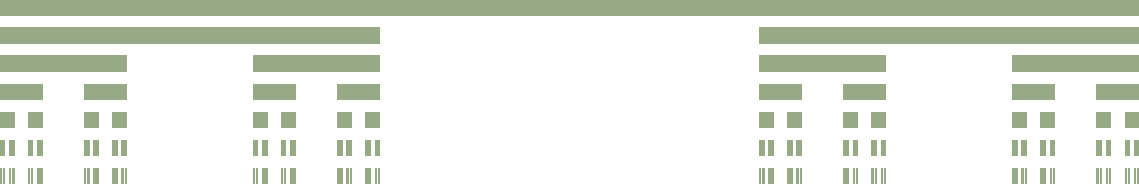
\includegraphics[width=16cm]{./attachment/cantor_set.pdf}
	\caption{Cantor集构造过程的示意图, 图源Wikipedia}
\end{figure}

Cantor集的构造过程用开集描述就是: 在第$n$次操作去掉(为了好写, 下面的开区间是包含已经去掉的部分的)$$I_n^1 = \big( \frac{1}{3^n},\frac{2}{3^n} \big), \quad  \cdots ,\quad I_n^k = \big( \frac{3k-2}{3^n},\frac{3k-1}{3^n} \big),\quad  \cdots , \quad I_n^{3^{n-1}} = \big( \frac{3^n-2}{3^n},\frac{3^n-1}{3^n} \big). $$

在分析Cantor集的性质之前, 需要定义: 

\begin{definition}{零测集}
	称一个集合$E \subseteq \R$是\textit{零测集}(null set), 如果对任意$\varepsilon >0$都存在至多可数个开区间组成的开覆盖$\{ I_n \}_{n \geq 1}$使得$\sum_{n=0}^{\infty} |I_n|<\varepsilon$. 
\end{definition}
\begin{remark}
	零测集的概念在Riemann积分部分还要使用. 
\end{remark}

无处稠密集的定义如同字面: 称$E$在$X$中无处稠密, 若对任意$x \in X$都存在邻域$U(x)$与$E$无交. 

\begin{proposition}{Cantor集的性质}
	Cantor集: 
	
	1) 是有限闭集(从而是紧集, 列紧集);\qquad 2) 是无处稠密集;
	
	3) 没有孤立点(这样的闭集称作完备集);\qquad 4) 是不可数集;\qquad 5) 是零测集. 
\end{proposition}
\begin{proof}
	(1) 由于$C_n$都是闭集, 可知$\mathcal{C}$也是闭集. 另外显然$\mathcal{C} \subseteq [0,1]$有限. 
	
	(2) 对任意$x \in [0,1]$, 显然存在足够大的$n,k$使得$x \in I_n^k$. 
	
	(3) 对任意$x \in \mathcal{C}$, 设$N$满足对任意$n>N$, $x \in C_N$. 特别地对每个$n$取$I_n$是包含$x$的闭区间, 再从$I_n$任取$x_n \neq x$, 那么$x_n \to x$. 
	
	(4) \underline{\textbf{证法一}}(直观但不够严谨)~~利用三进制来描述Cantor集的构造就是: 第$n$次操作去掉开区间$$I_n^k =  (0.a_1\cdots a_{n-1}1, 0.a_1\cdots a_{n-1}2),$$其中$0.a_1\cdots a_{n-1}=\frac{k}{3^{n-1}}$, $k$遍历$1,\cdots ,3^{n-1}$. 这就是说, $\mathcal{C} = \{ x:x\textit{的三进制表示中只有$0$或$2$} \}$. 将$\mathcal{C}$中的数的$2$全部变成$1$, 即得$\mathcal{C}$与$[0,1]$等势. 
	
	\underline{\textbf{证法二}}~~假设$\mathcal{C}$可数, 记$\mathcal{C} = \{ x_1,\cdots ,x_n,\cdots \}$. 下面归纳构造开区间列$\{ I_n \}$: 取$I_1 \subseteq [0,1]$使得$x_1 \in I_1$. 取$I_{n+1}$满足$$\overline{I_{n+1}} \subseteq I_n,\qquad x_n \notin \overline{I_{n+1}},\qquad I_{n+1} \cap \mathcal{C} \neq \varnothing .$$
	其中$I_{n+1} \cap \mathcal{C} \neq \varnothing$是由(3)保证的. 定义$K_n = \overline{I_n} \cap \mathcal{C}$, 则有紧集套$K_1 \supseteq \cdots \supseteq K_n \supseteq \cdots$, 于是$\cap_{n \geq 1}K_n \neq \varnothing$. 但是这与$x_n \notin K_{n+1}$矛盾. 
	
	(5) 任何一个$C_n$都能够覆盖$\mathcal{C}$, 而$|C_n| = 2^n \cdot \frac{1}{3^n} = \big( \frac{2}{3} \big)^n \to 0$, 因此$\mathcal{C}$是零测集. 
\end{proof}
\begin{remark}
	使用无限小数做证明的缺点在于: 例如$1/3$的三进制表示可以为$0.022\cdots$, 也可以为$0.1$, 我们需要人为约定只应用第一种情况. 
\end{remark}










